\documentclass[11pt]{article}
\usepackage{graphicx}
\usepackage{amsmath}
\usepackage{geometry}
\usepackage{caption}
\geometry{margin=1in}

\title{Image Analysis and Processing Report}
\author{Mahla Entezari}
\date{November 2023}

\begin{document}

\maketitle

\section{Introduction}
This report presents the analysis and processing of an image using Python. The purpose of this project was to manipulate and analyze an image, potentially involving operations like filtering, transformation, or enhancement. The project was implemented in a Jupyter Notebook, as provided in \texttt{Matrix.ipynb}.

\section{Original Image}
The original image used for processing is a scenic photograph of a landscape, as shown in Figure \ref{fig:original}. This image is used as the base for any modifications or processing steps applied during the project.

\begin{figure}[h!]
    \centering
    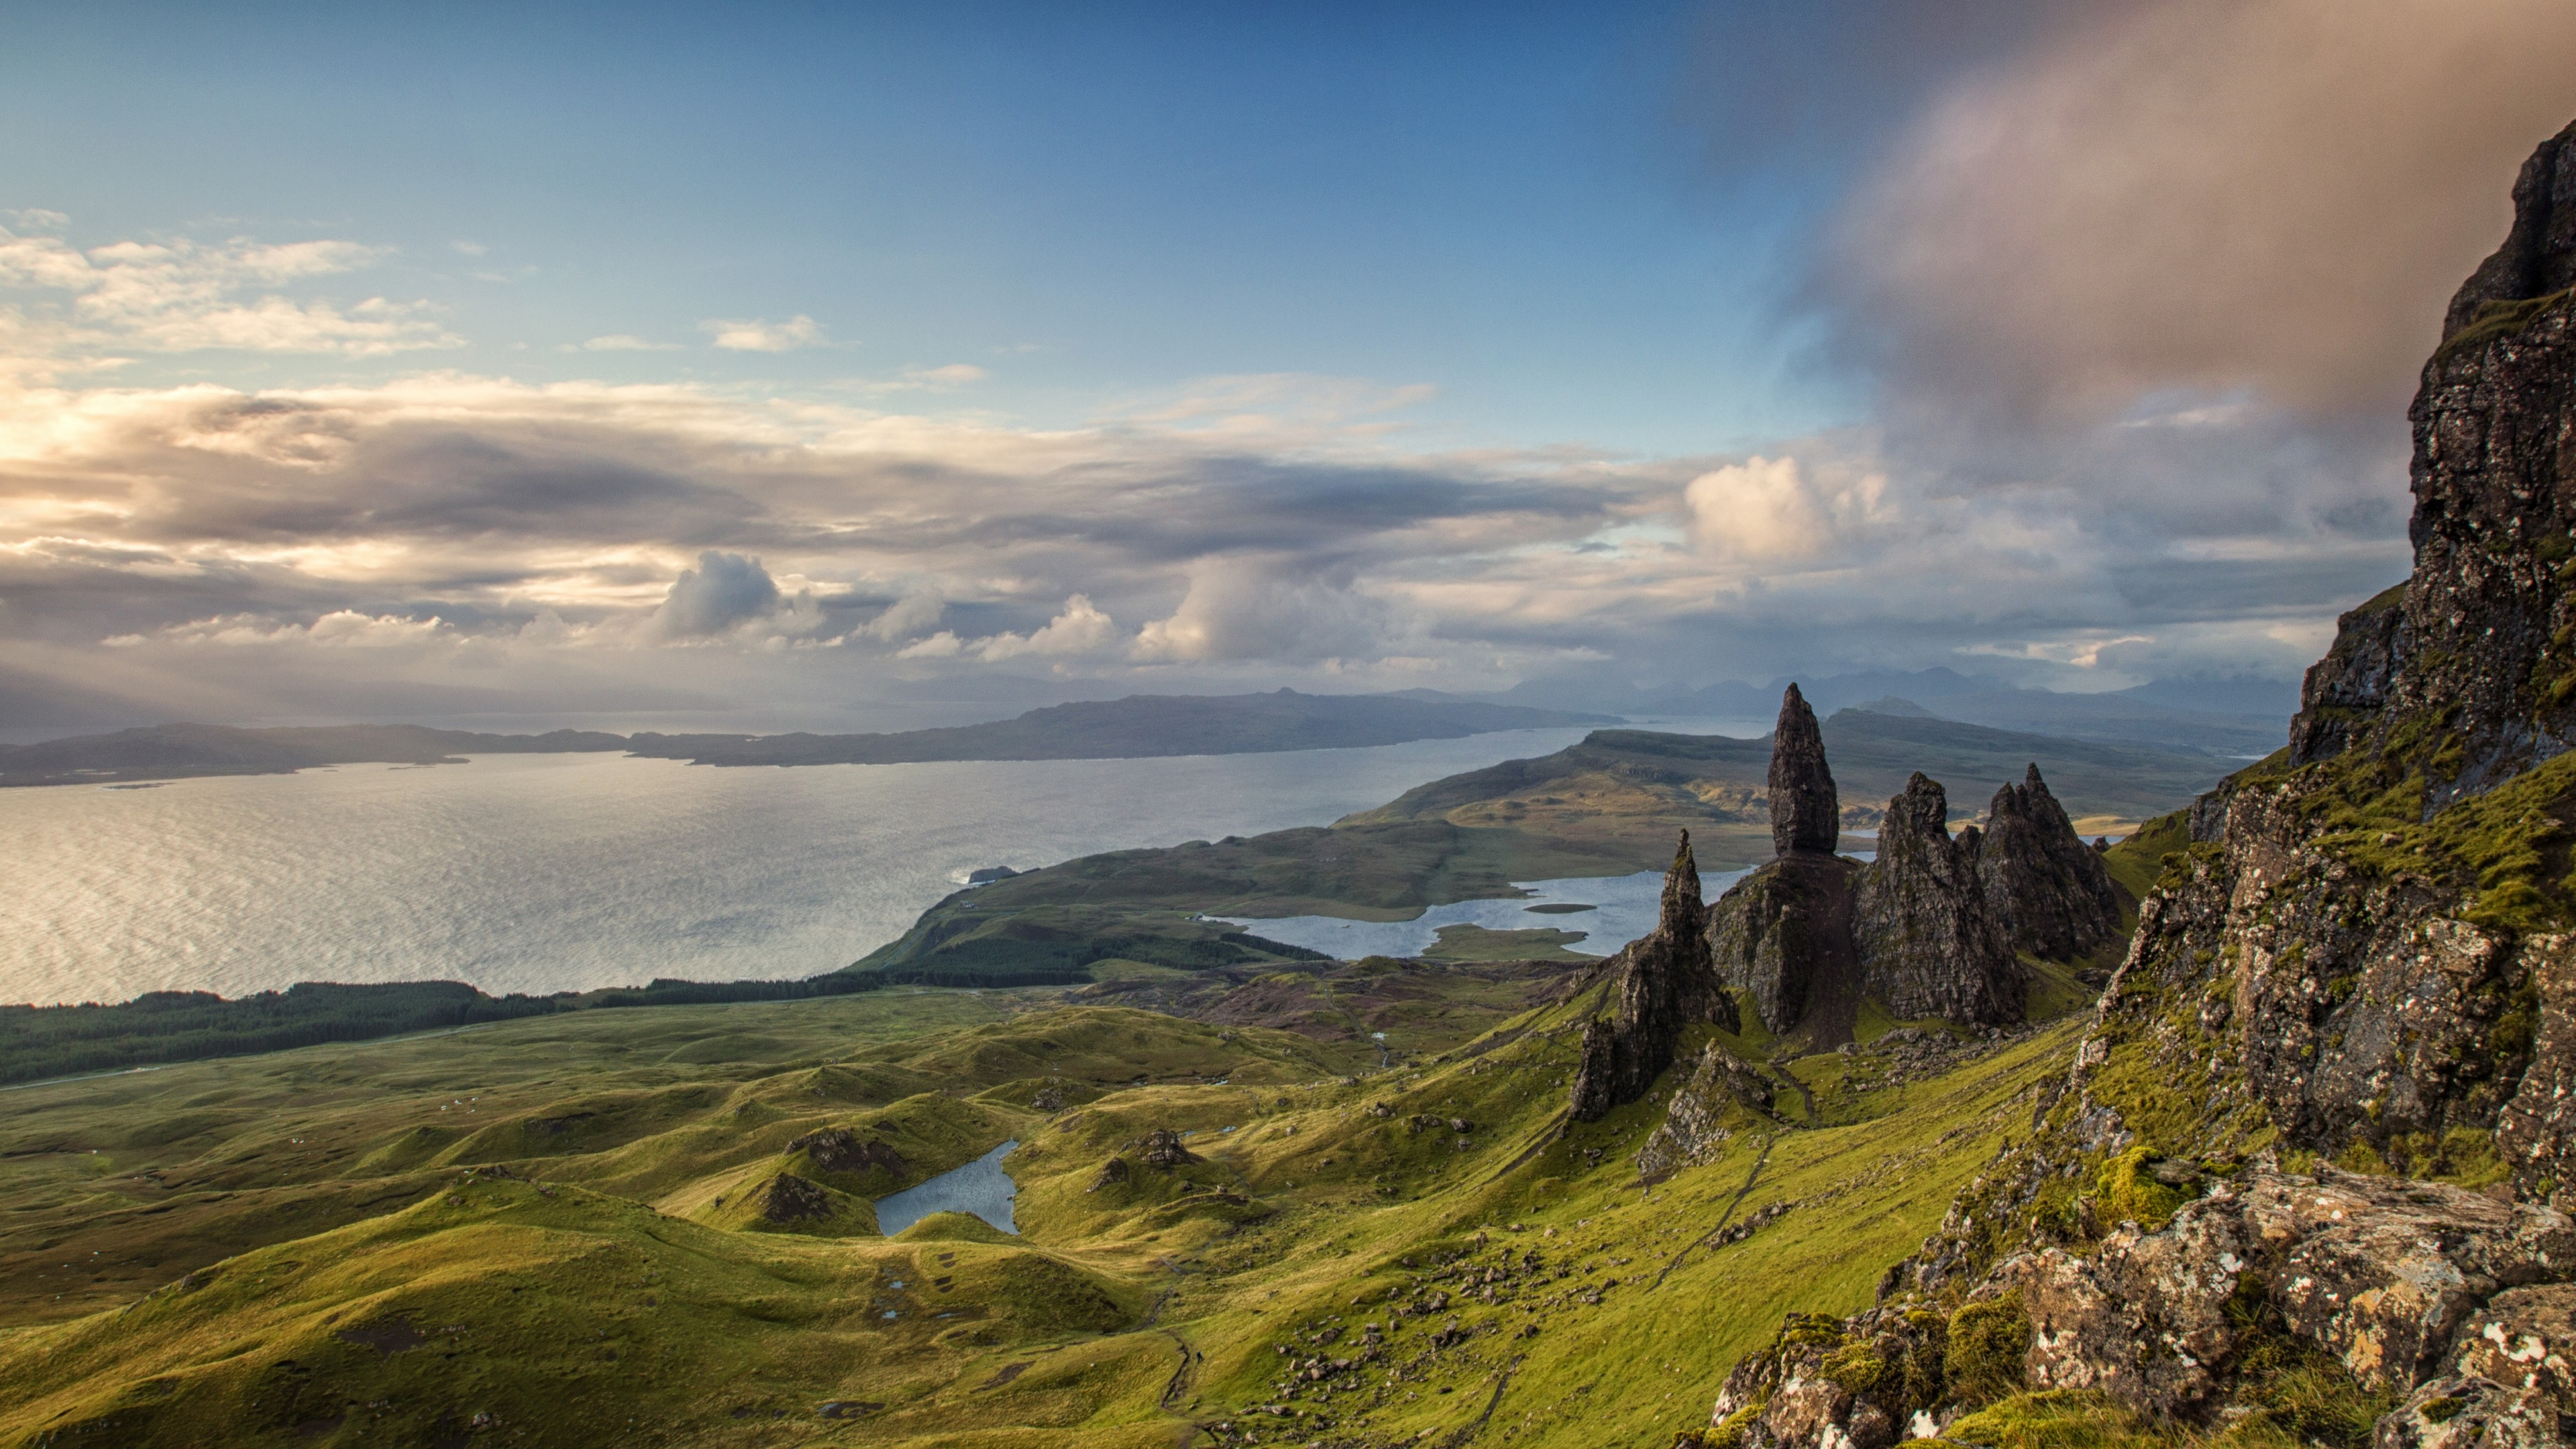
\includegraphics[width=\textwidth]{wallpaper.jpg}
    \caption{Original Landscape Image}
    \label{fig:original}
\end{figure}

\section{Processed Image}
After applying image processing techniques, the resulting image is shown in Figure \ref{fig:processed}. The operations performed on the image were implemented in the accompanying notebook, which may include transformations like cropping, filtering, edge detection, or enhancements.

\begin{figure}[h!]
    \centering
    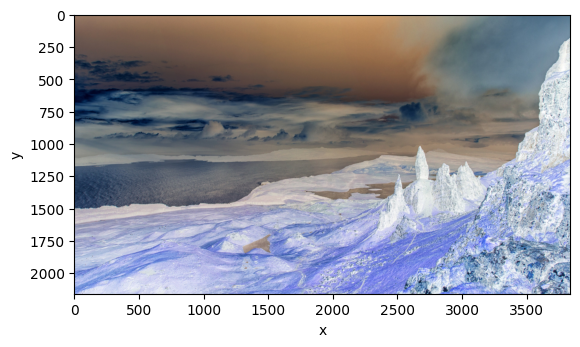
\includegraphics[width=\textwidth]{output.png}
    \caption{Processed Image}
    \label{fig:processed}
\end{figure}

\section{Methodology}
The analysis was conducted using a Python-based Jupyter Notebook (\texttt{Matrix.ipynb}). Key libraries likely used include \texttt{numpy}, \texttt{matplotlib}, and \texttt{opencv-python}. The workflow typically involves the following steps:
\begin{itemize}
    \item Reading the image using OpenCV or Matplotlib
    \item Applying transformations or processing
    \item Displaying and saving the final result
\end{itemize}

\section{Conclusion}
The project demonstrated basic image processing techniques using Python. The contrast between the original and processed images highlights the effectiveness of the operations used. Further work could involve more advanced processing such as object detection or segmentation.

\end{document}
